\documentclass[10pt]{article}
\usepackage{fancyhdr}
\usepackage{amsmath}
\usepackage{graphicx}
\pagestyle{fancy}
\headheight 35pt
\parskip 10pt \parindent 0pt 
\lhead{Classical Mechanics HW 1}
\chead{Andrei Ilyashenko}
\rhead{09-08-2010}
\cfoot{\thepage}

\begin{document}
%%%%%%%%%%%%%%%%%%%%%%%%%%%%%%%%%%%%%%%%%%%%%%%%%%%%%%%%%%%%%%%%%%%%%%%%%%%%%%%%%%%%
\textbf{Derivation 1}\\
For a single particle, with constant mass, the equation of motion is
\begin{align*}
  \vec F &= m\vec a
\end{align*}
If we differentiate the kinetic energy with respect to time, we get
\begin{align*}
  \frac{d T}{d t} &= \frac{d}{d t}\frac{1}{2}m\vec v\cdot\vec v\\
  &= m\vec v\cdot\vec a+\frac{1}{2}\dot m\vec v\cdot\vec v
\end{align*}
Since, $m$ is constant, the second term is 0, and from the equation of motion, 
we know that $\vec F=m\vec a$, so the equation above becomes
\begin{align*}
  \frac{dT}{dt} &= \vec F\cdot\vec v.
\end{align*}

If, $m$ is not constant, then the equation of motion is
\begin{align*}
  \vec F &= m\vec a + \dot m\vec v,
\end{align*}
and differentiating $mT$ with respect to time gives
\begin{align*}
  \frac{d mT}{d t} &= \frac{d}{d t}\frac{1}{2}m^2\vec v\cdot\vec v\\
  &= m^2\vec v\cdot\vec a+m\dot m\vec v\cdot\vec v\\
  &= m\vec v\cdot(m\vec a+\dot m\vec v).
\end{align*}
From the equation of motion, it is clear that the term in parenthesis is just the force, so the equation becomes
\begin{align*}
  \frac{d mT}{dt} &= \vec F\cdot (m\vec v) = \vec F\cdot\vec p.
\end{align*}
\textbf{Exercise 12}\\
First, we need to determine the work needed to move an object from the surface of the earth to infinitely far away from it (i.e. escape the earth's gravitational field).  This is given by the following integral
\begin{align*}
  \int_{r=R}^{\infty} -\frac{GmM}{r^2}dr &= \frac{GmM}{R}.
\end{align*}
So, the potential energy of a particle of mass m on the surface of the earth is $-\frac{GmM}{R}$.  Thus, a particle must have a kinetic energy of at least $\frac{GmM}{R}$ in order to escape from the earth's gravity.  This corresponds to a velocity of $\sqrt{\frac{2GM}{R}}\approx11.187 km/s$.\\
\textbf{Exercise 13}\\
Newton's second law states
\begin{align*} F_{ext} = \frac{dP}{dt} \end{align*}
So, in order to apply newton's second law to the rocket, we need to determine 
the momentum $P$ of the rocket-fuel system at an arbitrary time $t$.  This
momentum will be the sum of the momentum of the rocket plus the unspent fuel
and the momentum of the ejected fuel.  The momentum of the rocket is $mv$, 
where $m(t)$ is the mass of the rocket and $v(t)$ is the velocity of the rocket
relative to the earth.  To get the momentum of the ejected fuel, we need to
integrate $(v-v')\dot m$ where $v'$ is the velocity of the fuel relative to
the rocket (so $v-v'$ is the velocity of the fuel relative to the earth) and
$\dot m$ is assumed to be constant.  So, the momentum of the rocket-fuel system
at time $t$ is
\begin{align*}
  P(t) &= m(t)v(t) + \int_0^t (v-v')\dot m dt\\
       &= mv + \dot m(x-v't).
\end{align*}
Now, all we need is to determine the external force.  The problem says to assume
a uniform gravitational field, so then the external force is $-mg$.  Substituting
these expressions into Newton's second law gives
\begin{align*}
  F_{ext} &= \frac{dP}{dt}\\
  -mg &= \dot mv + m\dot v + \dot m(v-v')\\
  -mg &= m\dot v - \dot mv'\\
  m\dot v &= -mg - \dot mv'\\
  \dot v &= -g - \frac{\dot m}{m}v',
\end{align*}
which is the expected result.  Now, we integrate both sides from time 0 to time $T$, 
\begin{align}
  \int_0^T\dot vdt &= \int_0^T(-g - \frac{\dot m}{m}v')dt\nonumber\\
  v_f-v_i &= -gT - v'ln\left( \frac{m_e}{m_i} \right).
  \label{eq:ex13}
\end{align}
where $m_i$ is the initial mass, $m_e$ is the mass of the empty rocket, and
lets say $m_f$ is the mass of the fuel.  Notice that $T=m_f/\dot m$ assuming
the rocket expends all of its fuel.  Now let $r=m_f/m_e$, and then we can
rewrite $m_e/m_i$ as $1/(1+r)$, and $m_f/m_e$ as $r/(1+r)$.  Now, the problem
asks to determine the fuel to rocket mass ratio ($r$) needed for a rocket to
accelerate from rest to 11.2 km/s with an exhaust speed of 2.1 km/s and a mass
loss rate of $1/60 m_i$. Substituting these values into eq. \ref{eq:ex13} gives
\begin{align*}
  11.2\mathrm{km/s} &= \left( -60g - 2.1\times\ln\left( \frac{1}{1+r} \right)\right)\mathrm{km/s}\\
\end{align*}
With $60g=60\times.0098 \mathrm{km/s}$, this equation can be solved numerically to get $r=273.056$.\\
\textbf{Exercise 14}\\
This is a two dimensional problem, and the generalized coordinates $\theta$ and $\phi$ are given in fig. \ref{fig:ex14}
\begin{figure}[h!]
    \centering
    \includegraphics[width=0.7\textwidth]{Ex14.png}
    \caption{A graph showing the generalized coordinates $\theta$, and $\phi$.  The two balls of mass $m$ are held together by a rod of length $L$, the center of which is fixed to a circle of radius $a$.}
  \label{fig:ex14}
\end{figure}
The position of the center of the rod in terms of the generalized coordinate $\theta$ is
\begin{align*}
  \vec{rod} &= a(\cos(\theta),\sin(\theta))
\end{align*}
and the positions of the two masses are
\begin{align*}
  \vec{r_1} &= \vec{rod}+\frac{L}{2}(\cos\phi, \sin\phi)\\
  \vec{r_2} &= \vec{rod}-\frac{L}{2}(\cos\phi, \sin\phi)
\end{align*}
so, the velocities are
\begin{align*}
  \vec{v_1} &= \frac{\partial}{\partial t} \vec{r_1} = a\dot\theta(-\sin(\theta),\cos(\theta)) + \frac{L}{2}\dot\phi(-\sin(\phi),\cos(\phi))\\
  \vec{v_2} &= \frac{\partial}{\partial t} \vec{r_2} = a\dot\theta(-\sin(\theta),\cos(\theta)) + \frac{L}{2}\dot\phi(\sin(\phi),-\cos(\phi)).
\end{align*}
And, the total kinetic energy is
\begin{align*}
  T &= \frac{1}{2}m\left( \vec{v_1}\cdot\vec{v_1} + \vec{v_2}\cdot\vec{v_2} \right)\\
  &= \frac{1}{2}m\left( \left( a\dot\theta\sin\theta+\frac{L}{2}\dot\phi\sin\phi \right)^2 + \left( a\dot\theta\cos\theta+\frac{L}{2}\dot\phi\cos\phi \right)^2 \right.+\\
  &\hspace{37pt}\left.\left( a\dot\theta\sin\theta-\frac{L}{2}\dot\phi\sin\phi \right)^2 + \left( a\dot\theta\cos\theta-\frac{L}{2}\dot\phi\cos\phi \right)^2  \right) \\
  &= \frac{1}{2}m\left( 2a^2\dot\theta^2\sin^2\theta+\frac{2L^2}{4}\dot\phi\sin^2\phi+2a^2\dot\theta^2\cos^2\theta+\frac{2L^2}{4}\dot\phi\cos^2\phi \right)\\
  &= m(a^2\dot\theta^2+\frac{L^2}{4}\dot\phi^2).
\end{align*}
\textbf{Exercise 18}\\
The equations of motion for the Lagrangian,
\begin{align*}
  L' = \frac{m}{2}\left( a\dot x^2 + 2b\dot x \dot y + c\dot y^2 \right) - \frac{K}{2}\left( ax^2 + 2bxy + c y^2 \right),
\end{align*}
are
\begin{align*}
  \frac{d}{dt}\frac{\partial L'}{\partial \dot x} -  \frac{\partial L'}{\partial x} &= 0\\
  ma\ddot x + mb\ddot y + Ka x + Kby &= 0\\
  \frac{d}{dt}\frac{\partial L'}{\partial \dot y} -  \frac{\partial L'}{\partial y} &= 0\\
  mc\ddot y + mb\ddot x + Kc y + Kbx &= 0.
\end{align*}
If we let $\vec a = (\ddot x, \ddot y)$ and $\vec r = (x,y)$, then the
equation of motion becomes
\begin{align*}
  m\vec a\cdot(a,b) &= -K\vec r\cdot(a,b)\\
  m\vec a\cdot(b,c) &= -K\vec r\cdot(b,c)\\
\end{align*}
Remember that we can always multiply or divide an equation by a non-zero number
without invalidating it.  So, if we were to divide the first equation by 
$\sqrt{a^2+b^2}$, and the second by $\sqrt{b^2+c^2}$, we would get
\begin{align*}
  m\vec a\cdot\hat{(a,b)} &= -K\vec r\cdot\hat{(a,b)}\\
  m\vec a\cdot\hat{(b,c)} &= -K\vec r\cdot\hat{(b,c)}\\
\end{align*}
Where the hat signifies that the vector is a unit vector pointing in the same
direction.  Now, it is clear that the first equation relates the acceleration
along the $(a,b)$ direction to the position along the same direction, and
the second equation does the same in the $(b,c)$ direction.  So, if we define
new coordinates through a point transformation
\begin{align*}
  \tilde x &= \frac{ax+by}{\sqrt{a^2+b^2}} = r\cdot\hat{(a,b)}\\
  \tilde y &= \frac{bx+cy}{\sqrt{b^2+c^2}} = r\cdot\hat{(b,c)}\\
  \\
  x &= \frac{\tilde y b \sqrt{b^2+c^2} - \tilde x c \sqrt{a^2+b^2} }{\sqrt{b^2-ac}}\\
  y &= \frac{\tilde x b \sqrt{a^2+b^2} - \tilde y a \sqrt{b^2+c^2} }{\sqrt{b^2-ac}}\\
\end{align*}
This point transformation basically exchanges the $x$ and $y$ axis for new axis
pointing in the $(b,c)$ and $(a,b)$ directions.  If we apply this
transformation to the equations of motion, we get
\begin{align*}
  m\vec a\cdot\hat{(a,b)} &= -K\vec r\cdot\hat{(a,b)}\\
  m\vec a\cdot\hat{(b,c)} &= -K\vec r\cdot\hat{(b,c)}\\
  \\
  m\ddot{\tilde x} &= -k \tilde x\\
  m\ddot{\tilde y} &= -k \tilde y,
\end{align*}
and it becomes clear that this Lagrangian describes a spring-like central 
force system, where $\vec F = -K \vec{r}$.  The usual Lagrangian for this 
system is
\begin{align*}
  L = \frac{m}{2}\left( \dot x^2 + \dot y^2 \right) - \frac{K}{2}\left( x^2 + y^2 \right),
\end{align*}
and it is related to the given Lagrangian by the point transformation 
discussed above.  The two cases that the problem asks you to look at:
$a=0=c$, and $b=0, a=-c$ correspond to no change in the axis, since 
the new axis are $(0,1), (1,0)$ and $(1,0), (0,1)$ respectively.  Also, now
the condition on $b^2-ac$ can be reinterpreted as the condition that the
new axes $(a,b)$, and $(b,c)$, must not be parallel, since then the transformation
would not be one to one.
\begin{align*}
 \hat{(a,b)} &\neq \hat{(b,c)}\\
 \sqrt{b^2+c^2}(a,b) &\neq \sqrt{a^2+b^2}(b,c)\\
 \\
 \sqrt{b^2+c^2}a &\neq \sqrt{a^2+b^2}b\\
 \sqrt{b^2+c^2}b &\neq \sqrt{a^2+b^2}c\\
 \\
 (b^2+c^2)a &\neq (a^2+b^2)b\\
 (b^2+c^2)b &\neq (a^2+b^2)c\\
 \\
 \frac{a}{b} &\neq \frac{b}{c}\\
 b^2 &\neq ac\\
 b^2-ac &\neq 0.
\end{align*}
In fact, it is even apparent from the form of the point transformation that
$b^2-ac &\neq 0$ since this term appears in the denominator.

\end{document}
